\chapter{Evaluation}\label{C:eval}

\section{Accuracy Testing}
\par To test the accuracy of the device, a loopback test was performed with different length of cables. This was 
setup so that there was no switch between two ethernet measurement ports, only an ethernet cable. The test is to 
ensure that the device is measuring the latency correctly, and able to detect the latency present in a specific 
length of cable. Latency measured from the device can be compared with the theoretical value of the latency which 
can be calculated using the following formula:

\[Latency = \frac{L}{cV_f}\]

\par Where L is the length of the cable, c is the speed of light (299,792,458 m/s) and V\textsubscript{f} is 
velocity factor of ethernet cables (0.65). 

\par A very short cable (4 cm) was used to measure the processing time, a constant added to every measurement. 
This processing time is the result of both Ethernet Phy’s converting between the two protocols (Differential Pairs 
and RGMII). Performing measurements with the short cable produced a mean value of 440 ns where 0.2095 ns of the 
measurement is attributed to the delay present in the cable.

\par This processing time is then removed from subsequent tests, making the latency values produced by the device 
purely the latency present in the cable. The goal from the tests is to ensure that the device is accurate to within
4 ns, which is the smallest interval of time that can be measured.

\par Tests were done with cables spanning 2 m, 3 m and 25 m long. These provided enough of a delay to measure with the
device, and enough data to characterise the accuracy of what cables are used. The measured value was plotted with 
the theoretical values of what delay would be present in the cable. To obtain the delay measurement, the test was 
run for 20 seconds on the device, with a packet transmission frequency of 500 packets per second. The mean value
of all packet latency measurements for that cable were then plotted versus the length of the cable.

\begin{figure}[H]
    \begin{center}
        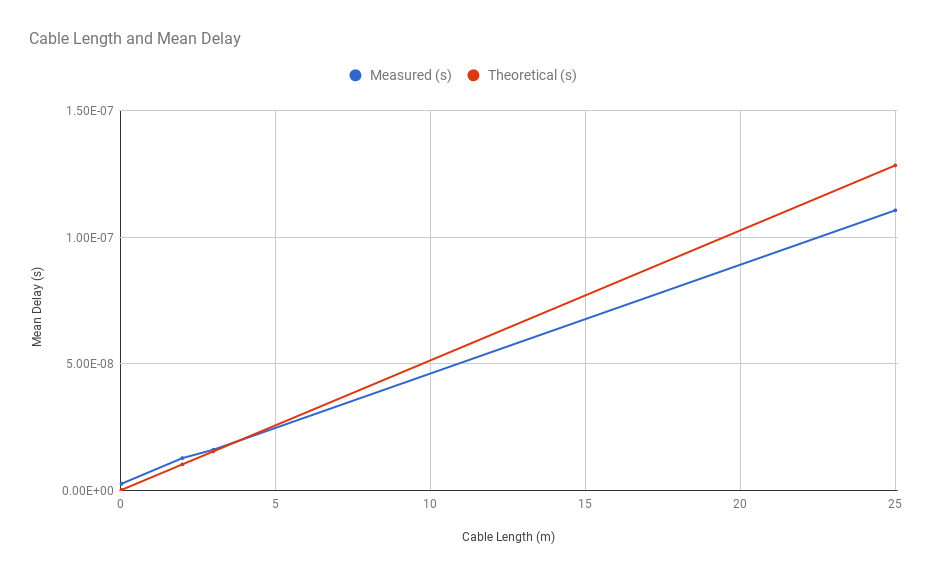
\includegraphics[keepaspectratio,width=15cm]{Images/CableTesting}
        \caption{Results from Accuracy Measurements}
        \label{fig:accuracyMeasurements}
    \end{center}
\end{figure}

\par As shown in ~\ref{fig:accuracyMeasurements}, the results from the device show a linear trend in latency due to 
length of the cable. The gradient difference of the theoretical line can be attributed to the fluctuation in 
velocity factor through the different cables.

\par The difference between the theoretical and measured value of the 25 m cable was 14 ns. This is not within the 
accuracy margin which was required, hence 2 m and 3 m cables are used for the reliablity tests as the difference was below 2 ns.

\section{Reliability Testing}

\par To test reliability of the device, repeated tests were performed to show that results would stay consistent
from test to test. As the goal of the project was to measure the latency in network swtiches, these tests were to 
measure the latency through a network switch and provide repeatable results. These results did not neccessarily have
to be accurate, as the accuracy was determined in the test in accuracy testing, hence these results are only to 
measure the reliability.

\par Results from the tests were compared to an existing DPDK software based latency measurement method. This was 
run on two separate machines which had clocks synchronoised using PTP protocol and as a result, the timings varied 
significantly. This comparision was to show that the software based methods have flexibility that hardware methods
are missing while also performing unreliably. The DPDK based system was compared to the FPGA based device by producing
a packet on one machine, then sending the packet through the network switch to arrive at the other machine, and the
time delta is returned from both machines. The FPGA device also performed the same task with the same cables, but 
the two connections arrived at the same machine.
